\pagebreak
\section*{注意力可视化}\label{sec:viz-att}
\begin{figure*}[h]
{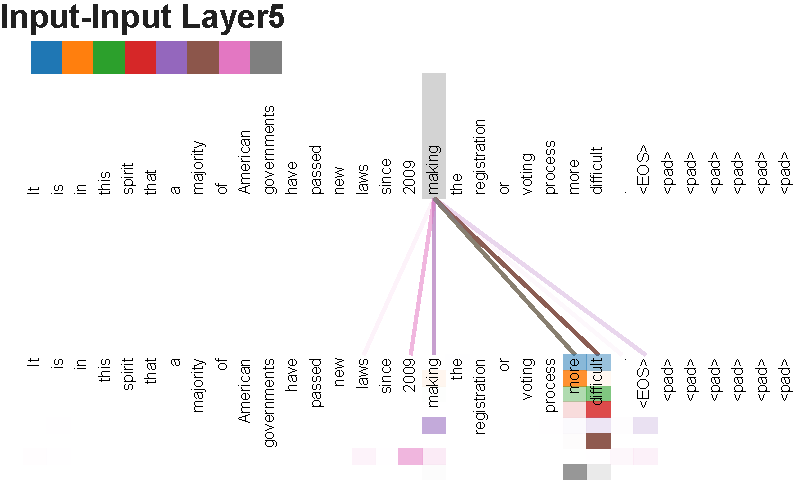
\includegraphics[width=\textwidth, trim=0 0 0 36, clip]{./vis/making_more_difficult5_new.pdf}}
\caption{注意力机制跟踪编码器第 5 层自注意力中长距离依赖的示例。许多注意力头关注动词 `making` 的远程依赖，完成短语 `making...more difficult`。这里只显示了单词 `making` 的注意力。不同颜色代表不同的头。最好在彩色显示器上查看。}
\end{figure*}

\begin{figure*}
{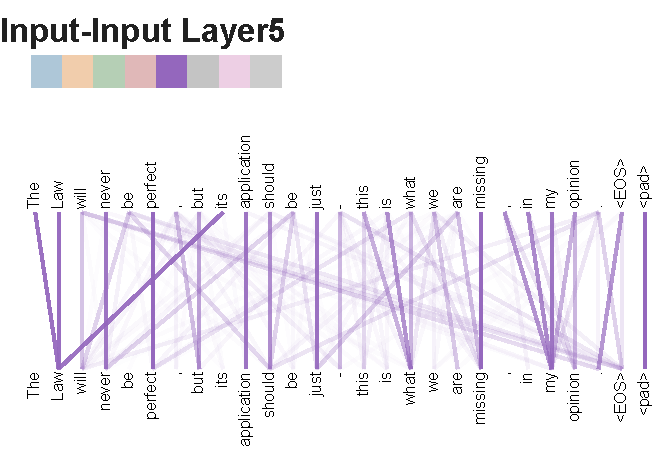
\includegraphics[width=\textwidth, trim=0 0 0 45, clip]{./vis/anaphora_resolution_new.pdf}}
{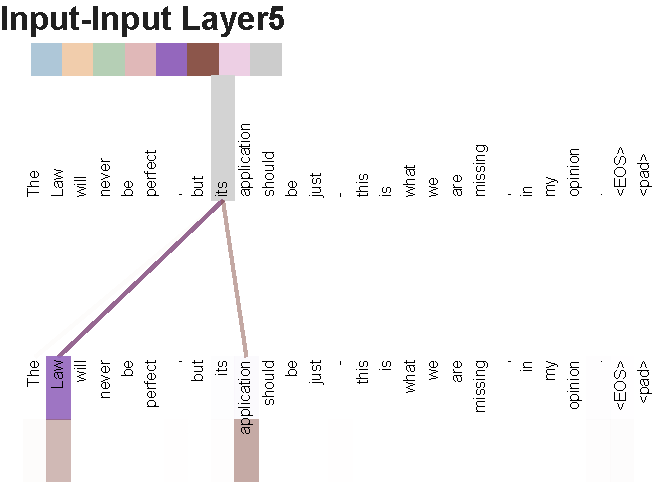
\includegraphics[width=\textwidth, trim=0 0 0 37, clip]{./vis/anaphora_resolution2_new.pdf}}
\caption{两个注意力头，也在第 5 层，显然参与指代消解。上图：头 5 的完整注意力。下图：只来自单词 `its` 对注意力头 5 和 6 的隔离注意力。注意这个单词的注意力非常尖锐。}
\end{figure*}

\begin{figure*}
{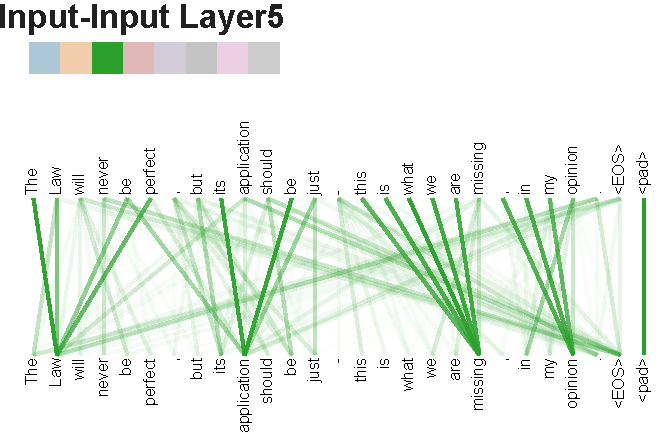
\includegraphics[width=\textwidth, trim=0 0 0 36, clip]{./vis/attending_to_head_new.pdf}}
{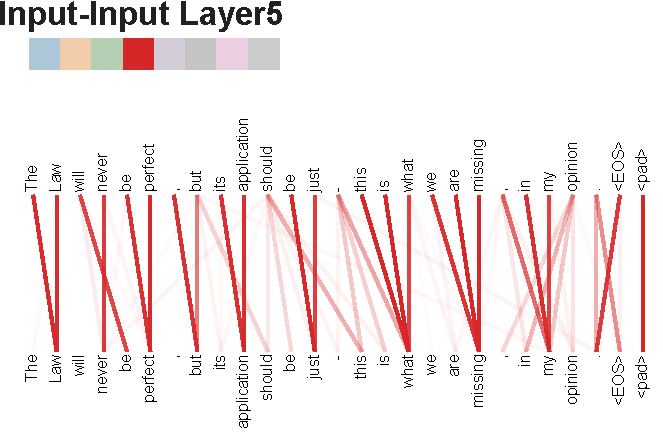
\includegraphics[width=\textwidth, trim=0 0 0 36, clip]{./vis/attending_to_head2_new.pdf}}
\caption{许多注意力头表现出的行为似乎与句子结构有关。我们上面给出了两个这样的例子，来自编码器第 5 层自注意力的两个不同的头。这些头清楚地学会了执行不同的任务。}
\end{figure*}
